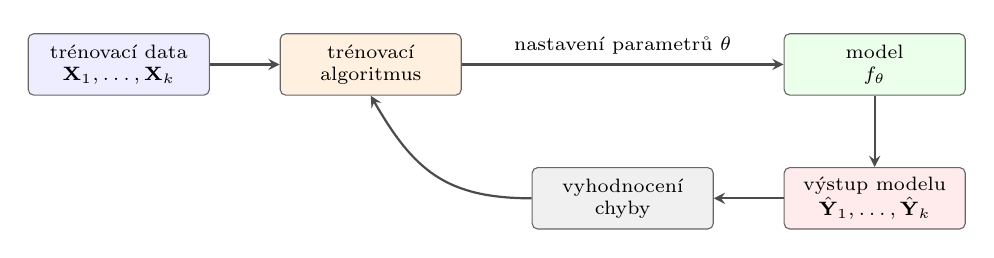
\begin{tikzpicture}[
    >=stealth,
    box/.style={
        draw=black!60,
        rounded corners=2pt,
        minimum width=2.3cm,
        minimum height=0.78cm,
        align=center,
        font=\scriptsize
    },
    smallbox/.style={
        draw=black!55,
        rounded corners=2pt,
        minimum width=1.95cm,
        minimum height=0.58cm,
        align=center,
        font=\scriptsize
    },
    arr/.style={->, thick, draw=black!70},
    braceup/.style={decorate,decoration={brace,amplitude=4pt}, thick}
]

    % Hlavní řetězec
    \node[box, fill=blue!7] (data) at (0,0)
        {trénovací data\\$\mathbf{X}_1,\dots,\mathbf{X}_k$};

    \node[box, fill=orange!12] (alg) at (3.2,0)
        {trénovací\\algoritmus};

    \node[box, fill=green!8] (model) at (9.6,0)
        {model\\$f_{\boldsymbol{\theta}}$};

    \node[box, fill=red!8] (pred) at (9.6,-1.7)
        {výstup modelu\\$\hat{\mathbf{Y}}_1,\dots,\hat{\mathbf{Y}}_k$};

    \node[box, fill=gray!12] (err) at (6.4,-1.7)
        {vyhodnocení\\chyby};

    % Šipky
    \draw[arr] (data) -- (alg);
    \draw[arr] (alg) -- node[above, font=\scriptsize]
        {nastavení parametrů $\boldsymbol{\theta}$} (model);
    \draw[arr] (model) -- (pred);
    \draw[arr] (pred) -- (err);

    \draw[arr]
        (err.west)
        to[out=180,in=-60,looseness=1.15]
        (alg.south);

\end{tikzpicture}
